%pdflatex Baylor_Fain_SMB_2021.tex && pdflatex Baylor_Fain_SMB_2021.tex
\PassOptionsToPackage{cmyk}{xcolor}
\documentclass{beamer}
%\documentclass[handout]{beamer}
\usepackage{xcolor}
\usepackage{colortbl}
\definecolor{AGreen}{HTML}{00ff00}
\usepackage[squaren]{SIunits}
\usepackage{xspace}
\usepackage{animate}
\usepackage{longtable}
\usepackage{makecell}
\setcellgapes{2pt}
\usepackage{tikz}
\usepackage{tkz-graph}
\usetikzlibrary{automata, positioning, arrows, shapes, snakes}
\tikzset{
    ->,  % makes the edges directed
    >=stealth, % makes the arrow heads bold
    node distance=3cm, % specifies the minimum distance between two nodes. Change if necessary.
    every state/.style={thick, fill=gray!10}, % sets the properties for each ’state’ node
    initial text=$ $, % sets the text that appears on the start arrow
}
\usetikzlibrary{shapes.arrows}
\tikzset{
    myarrow/.style={
        draw,
        fill=black,
        single arrow,
        minimum height=3.5ex,
        single arrow head extend=1ex
    }
}
\newcommand{\arrowup}{%
\tikz [baseline=-0.5ex]{\node [myarrow,rotate=90] {};}
}
\newcommand{\arrowdown}{%
\tikz [baseline=-1ex]{\node [myarrow,rotate=-90] {};}
}
\newcommand{\arrowright}{%
\tikz [baseline=-1ex]{\node [myarrow,rotate=0] {};}
}
\newcommand{\arrowleft}{%
\tikz [baseline=-1ex]{\node [myarrow,rotate=180] {};}
}
\newcommand{\arrowSW}{%
\tikz [baseline=-1ex]{\node [myarrow,rotate=-135] {};}
}
\newcommand{\arrowSE}{%
\tikz [baseline=-1ex]{\node [myarrow,rotate=-45] {};}
}
\newcommand{\arrowNE}{%
\tikz [baseline=-1ex]{\node [myarrow,rotate=45] {};}
}
\usetikzlibrary{automata, positioning, arrows}
\tikzset{
    ->,  % makes the edges directed
    >=stealth, % makes the arrow heads bold
    node distance=3cm, % specifies the minimum distance between two nodes. Change if necessary.
%    every state/.style={thick, fill=green!10}, % sets the properties for each ’state’ node
    initial text=$ $, % sets the text that appears on the start arrow
}

\def\firstcircle{(90:1.75cm) circle (2.5cm)}
\def\secondcircle{(210:1.75cm) circle (2.5cm)}
\def\thirdcircle{(330:1.75cm) circle (2.5cm)}


\graphicspath{{Figures/}}
\usepackage{pgfpages}




\setbeameroption{hide notes}  %Only slides
%\setbeameroption{show only notes} % Only notes
%\setbeameroption{show notes on second screen=right} % Both
%Make note
%\note[item]{}

% Give a slight yellow tint to the notes page
\setbeamertemplate{note page}{\pagecolor{yellow!5}\insertnote}\usepackage{palatino}

%\definecolor{APurple}{HTML}{860076}
%\definecolor{TCUPurple}{HTML}{454084}
%\definecolor{TCUPurple}{cmyk}{79,100,0,20}

\mode<presentation>
{
  \usetheme{Singapore}
  \usecolortheme[named=violet]{structure}
  % or ...

  \setbeamercovered{invisible}
  % or whatever (possibly just delete it)
}

\usepackage[english]{babel}
% or whatever

\usepackage[latin1]{inputenc}
% or whatever

\usepackage{times}
\usepackage[T1]{fontenc}
% Or whatever. Note that the encoding and the font should match. If T1
% does not look nice, try deleting the line with the fontenc.

\setbeamertemplate{footline}{
  \hfill%
  \usebeamercolor[fg]{page number in head/foot}%
  \usebeamerfont{page number in head/foot}%
  \setbeamertemplate{page number in head/foot}[framenumber]%
  \usebeamertemplate*{page number in head/foot}\kern1em\vskip2pt%
}

\makeatletter
\let\beamer@writeslidentry@miniframeson=\beamer@writeslidentry%
\def\beamer@writeslidentry@miniframesoff{%
  \expandafter\beamer@ifempty\expandafter{\beamer@framestartpage}{}% does not happen normally
  {%else
    % removed \addtocontents commands
    \clearpage\beamer@notesactions%
  }
}
\newcommand*{\miniframeson}{\let\beamer@writeslidentry=\beamer@writeslidentry@miniframeson}
\newcommand*{\miniframesoff}{\let\beamer@writeslidentry=\beamer@writeslidentry@miniframesoff}
\makeatother

\usepackage{amsmath}
\usepackage{MnSymbol}
\usepackage{wasysym}
\usepackage{amssymb}
\usepackage{textcmds}
\usepackage{listings}
\definecolor{mGreen}{rgb}{0,0.6,0}
\definecolor{mGray}{rgb}{0.5,0.5,0.5}
\definecolor{mPurple}{rgb}{0.58,0,0.82}
\definecolor{backgroundColour}{rgb}{0.95,0.95,0.92}

\lstdefinestyle{CStyle}{
    backgroundcolor=\color{backgroundColour},   
    commentstyle=\color{mGreen},
    keywordstyle=\color{magenta},
    numberstyle=\tiny\color{mGray},
    stringstyle=\color{mPurple},
    basicstyle=\footnotesize,
    breakatwhitespace=false,         
    breaklines=true,                 
    captionpos=b,                    
    keepspaces=true,                 
    numbers=left,                    
    numbersep=5pt,                  
    showspaces=false,                
    showstringspaces=false,
    showtabs=false,                  
    tabsize=2,
    language=C
}

\setbeamertemplate{itemize item}[-]

\newcommand{\e}[1]{\ensuremath{\times10^{#1}}\xspace}

%\tiny
%\scriptsize
%\footnotesize
%\small
%\normalsize
%\large
%\Large
%\LARGE
%\huge
%\Huge
\title%
{{\LARGE Applying desktop GPUs to a hybrid ABM and PDM: model validation and rapid simulation of viral infections}}

\author%
{{Presented by:\\ \large Baylor Fain}}

\date%
{{\footnotesize July 15, 2021}}

\begin{document}

\begin{frame}
  \titlepage
\end{frame}

%\begin{frame}{Overview}
%  \tableofcontents%[pausesections]
%   %You might wish to add the option [pausesections]
%\end{frame}

%-----------------------------------------------------------------------------------
\section{Introduction}

\begin{frame}{Title break down}
\only<1>{Applying desktop GPUs to a hybrid ABM and PDM: model validation and rapid simulation of viral infections}
\only<2>{Applying desktop GPUs to a hybrid \underline{ABM} and PDM: model validation and rapid simulation of viral infections}
\only<3>{Applying desktop \underline{GPU}s to a hybrid \underline{ABM} and PDM: model validation and rapid simulation of viral infections}
\only<4->{Applying desktop \underline{GPU}s to a hybrid \underline{ABM} and PDM: model \underline{validation} and rapid simulation of viral infections}

\resizebox{1.0\linewidth}{!}{%
\begin{columns}[T]
\column{0.5\textwidth}
    \begin{center}
    \begin{itemize}
        \item<2-> ABM (Agent-based model)
        \item<3-> GPU (Graphics Processing Unit)
        \item<4-> Validation
    \end{itemize}
    \end{center}
\column{0.5\textwidth}
    \onslide<5->{%
    \begin{center}
    \resizebox{1.0\linewidth}{!}{%
    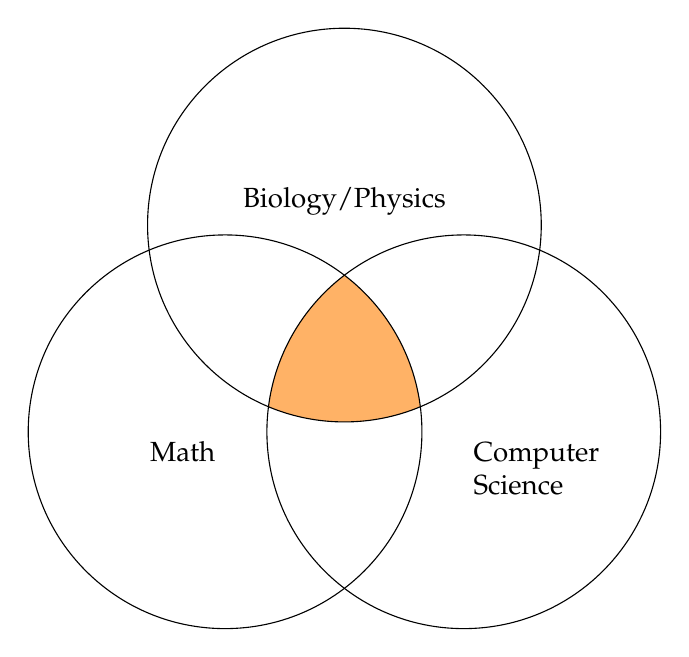
\begin{tikzpicture}
        \begin{scope}
        \clip \firstcircle;
        \clip \secondcircle;
        \clip \thirdcircle;
        \fill[orange!60] \thirdcircle;
        \end{scope}
        \draw \firstcircle node[text=black,above] {Biology/Physics};
        \draw \secondcircle node[text=black,below left] {Math};
        \draw \thirdcircle node[text=black,below right, align=left] {Computer\\Science};
    \end{tikzpicture}}
    \end{center}}
\end{columns}}
\end{frame}

\begin{frame}{Agent-Based Model}
The system in question is broken down into either naturally discrete segments or just smaller segments.
\resizebox{1.0\linewidth}{!}{%
\begin{columns}[c]
\column{0.5\textwidth}
    \begin{center}
        \onslide<2->{\resizebox{1.0\linewidth}{!}{\includegraphics{Fish}}}
    \end{center}
\column{0.5\textwidth}
    \begin{center}
        \onslide<3->{\resizebox{0.8\linewidth}{!}{\includegraphics{HeatDiffusion}}}
    \end{center}
\end{columns}}
\end{frame}

\begin{frame}{Why ABMs?}
\resizebox{1.0\linewidth}{!}{%
\begin{columns}[c]
\column{0.5\textwidth}
    \onslide<2->{
    \begin{center}
    
\begin{tikzpicture}
        \draw[fill=orange] (-1,2) to[bend left=50] (1,2) to[bend left=50] (-1,2);
        \draw[fill=orange] (1,2) -- (1.5,2.5) -- (1.3,2) -- (1.5,1.5) -- cycle;
        \draw[fill=white] (-0.4,2.1) circle (.15cm); 
        \draw[fill=blue] (-0.45,2.1) circle (.05cm);

        \draw[fill=red] (1,1) to[bend left=50] (3,1) to[bend left=50] (1,1);
        \draw[fill=red] (3,1) -- (3.5,1.5) -- (3.3,1) -- (3.5,.5) -- cycle;
        \draw[fill=white] (1.6,1.1) circle (.15cm); 
        \draw[fill=blue] (1.55,1.1) circle (.05cm);

        \onslide<3->{\draw (0,2) -- (2,1);}
    \end{tikzpicture}
    \end{center}}
\column{0.5\textwidth}
    \onslide<4->{
    \begin{center}
        \resizebox{0.8\linewidth}{!}{\includegraphics{plaques}}
    \end{center}}
\end{columns}}
\end{frame}

\begin{frame}{Published ABMs}
\begin{center}
\resizebox{1.0\linewidth}{!}{%
\begin{tabular}{lrr}
\hline
Articles & Cells Modeled & Number of Target Cells\\
\hline
\onslide<2->{Beauchemin et al.\ 2005} & \onslide<2->{1.2\e{5}}    & \onslide<3->{$\sim$1.2\e{6}}\\
\onslide<4->{Alvarado et al.\ 2018}   & \onslide<4->{4.0\e{4}}    & \onslide<5->{$\sim$1.2\e{6}}\\
\onslide<6->{Wodarz et al.\ 2014}     & \onslide<6->{2.0\e{4}}    & \onslide<7->{$\sim$2.4\e{5}}\\
\onslide<8->{Tong et al.\ 2015}       & \onslide<8->{6.0\e{5}}    & \onslide<9->{$\sim$1.0\e{9}}\\
\end{tabular}}

\vspace{2em}
\onslide<10->{All are at least an order of magnitude\\ \textcolor{red}{less than} the \underline{number of target cells}}

\end{center}
\end{frame}

\begin{frame}{Graphic Processes Unit}
A piece of computer hardware that contains a lot of processing units.
\resizebox{1.0\linewidth}{!}{%
\begin{columns}[T]
\column{0.5\textwidth}
    \begin{center}
    \onslide<2->{\resizebox{0.7\linewidth}{!}{\includegraphics{QuadroP4000}}}
    \begin{itemize}
        \item<3-> 1792 processing units
        \item<5-> 1.227 GHz
        \item<6-> 5.3 TFLOPS
            \begin{itemize}
                \item<7-> 5.3\e{12} FLOPS
            \end{itemize}
    \end{itemize}
    \end{center}
\column{0.5\textwidth}
    \vspace{1em}
    \begin{center}
    \onslide<4->{\resizebox{0.7\linewidth}{!}{\includegraphics{Xeon}}}
    \begin{itemize}
        \item<4-> 1 processing unit
        \item<5-> 3.6 GHz
        \item<6-> 442 GFLOPS
            \begin{itemize}
                \item<7-> 4.4\e{9} FLOPS
            \end{itemize}
    \end{itemize}
    \end{center}
\end{columns}}
\end{frame}

\begin{frame}{What do the GPUs do?}
\resizebox{1.0\linewidth}{!}{%
    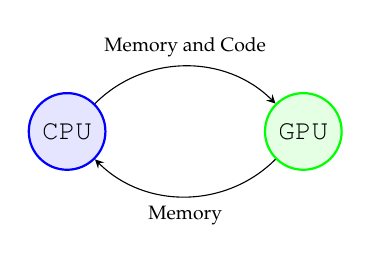
\begin{tikzpicture}
        \onslide<1->{\node[state, draw=blue, fill=blue!10] (H) {\texttt{CPU}};}
        \onslide<2->{\node[state, draw=green, fill=green!10, right of=H] (E) {\texttt{GPU}};}
        
        \onslide<2->{\draw   (H) edge[bend left=45] node[above] {\scriptsize Memory and Code} (E);}
        \onslide<3->{\draw   (E) edge[bend left=45] node[below] {\scriptsize Memory} (H);}
    \end{tikzpicture}}
\end{frame}

\begin{frame}[fragile]{Using the GPUs}
\begin{center}
    \texttt{CPU}
    \begin{lstlisting}[style=CStyle]
    for(int i=0; i<sizeof(array)/sizeof(array[0]); i++){
    array[i] = array[i] + 1;
    }\end{lstlisting}
\end{center}

\begin{center}
    \texttt{GPU}
    \begin{lstlisting}[style=CStyle]
    array_GPU[id] = array_GPU[id] + 1;\end{lstlisting}
\end{center}
\end{frame}

\begin{frame}[fragile]{\texttt{CPU} vs \texttt{GPU}}
\resizebox{1.0\linewidth}{!}{%
\begin{columns}[T]
\column{0.5\textwidth}
    \begin{center}
        \resizebox{0.3\linewidth}{!}{%
        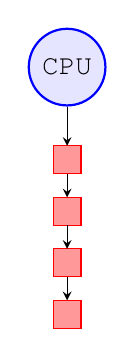
\begin{tikzpicture}[
            CODE/.style={regular polygon,regular polygon sides=4, draw, minimum size=0.5cm, inner sep=0pt, outer sep=0pt, draw=red, fill=red!40},
            ENDCODE/.style={regular polygon,regular polygon sides=4, draw, minimum size=0.5cm, inner sep=0pt, outer sep=0pt, draw=black, fill=black!40}]

            \onslide<1->{\node[state, minimum size=0.5cm, draw=blue, fill=blue!10] (CPU) {\texttt{CPU}};}
            \onslide<2->{\node[CODE, below=0.5cm of CPU] (C1) {};}
            \onslide<3->{\node[CODE, below=0.3cm of C1] (C2) {};}
            \onslide<4->{\node[CODE, below=0.3cm of C2] (C3) {};}
            \onslide<5->{\node[CODE, below=0.3cm of C3] (C4) {};}
                
            \onslide<2->{\draw   (CPU) edge node {} (C1);}
            \onslide<3->{\draw   (C1) edge node {} (C2);}
            \onslide<4->{\draw   (C2) edge node {} (C3);}
            \onslide<5->{\draw   (C3) edge node {} (C4);}
        \end{tikzpicture}}
    \end{center}
\column{0.5\textwidth}
    \begin{center}
        \resizebox{0.6\linewidth}{!}{%
        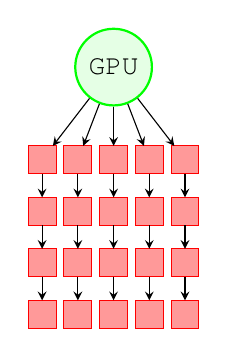
\begin{tikzpicture}[
            CODE/.style={regular polygon,regular polygon sides=4, draw, minimum size=0.5cm, inner sep=0pt, outer sep=0pt, draw=red, fill=red!40},
            ENDCODE/.style={regular polygon,regular polygon sides=4, draw, minimum size=0.5cm, inner sep=0pt, outer sep=0pt, draw=black, fill=black!40}]

            \onslide<7->{\node[CODE] (C1) {};}
            \onslide<7->{\node[CODE, right=0.1cm of C1] (C2) {};}
            \onslide<7->{\node[CODE, right=0.1cm of C2] (C3) {};}
            \onslide<7->{\node[CODE, right=0.1cm of C3] (C4) {};}
            \onslide<7->{\node[CODE, right=0.1cm of C4] (C5) {};}
            \onslide<6->{\node[state, above=0.5cm of C3, minimum size=0.5cm, draw=green, fill=green!10] (GPU) {\texttt{GPU}};}

            \onslide<8->{\node[CODE, below=0.3cm of C1] (C21) {};}
            \onslide<8->{\node[CODE, below=0.3cm of C2] (C22) {};}
            \onslide<8->{\node[CODE, below=0.3cm of C3] (C23) {};}
            \onslide<8->{\node[CODE, below=0.3cm of C4] (C24) {};}
            \onslide<8->{\node[CODE, below=0.3cm of C5] (C25) {};}

            \onslide<9->{\node[CODE, below=0.3cm of C21] (C31) {};}
            \onslide<9->{\node[CODE, below=0.3cm of C22] (C32) {};}
            \onslide<9->{\node[CODE, below=0.3cm of C23] (C33) {};}
            \onslide<9->{\node[CODE, below=0.3cm of C24] (C34) {};}
            \onslide<9->{\node[CODE, below=0.3cm of C25] (C35) {};}

            \onslide<10->{\node[CODE, below=0.3cm of C31] (C41) {};}
            \onslide<10->{\node[CODE, below=0.3cm of C32] (C42) {};}
            \onslide<10->{\node[CODE, below=0.3cm of C33] (C43) {};}
            \onslide<10->{\node[CODE, below=0.3cm of C34] (C44) {};}
            \onslide<10->{\node[CODE, below=0.3cm of C35] (C45) {};}
                
            \onslide<7->{\draw   (GPU) edge node {} (C1);}
            \onslide<7->{\draw   (GPU) edge node {} (C2);}
            \onslide<7->{\draw   (GPU) edge node {} (C3);}
            \onslide<7->{\draw   (GPU) edge node {} (C4);}
            \onslide<7->{\draw   (GPU) edge node {} (C5);}

            \onslide<8->{\draw   (C1) edge node {} (C21);}
            \onslide<8->{\draw   (C2) edge node {} (C22);}
            \onslide<8->{\draw   (C3) edge node {} (C23);}
            \onslide<8->{\draw   (C4) edge node {} (C24);}
            \onslide<8->{\draw   (C5) edge node {} (C25);}

            \onslide<9->{\draw   (C21) edge node {} (C31);}
            \onslide<9->{\draw   (C22) edge node {} (C32);}
            \onslide<9->{\draw   (C23) edge node {} (C33);}
            \onslide<9->{\draw   (C24) edge node {} (C34);}
            \onslide<9->{\draw   (C25) edge node {} (C35);}

            \onslide<10->{\draw   (C31) edge node {} (C41);}
            \onslide<10->{\draw   (C32) edge node {} (C42);}
            \onslide<10->{\draw   (C33) edge node {} (C43);}
            \onslide<10->{\draw   (C34) edge node {} (C44);}
            \onslide<10->{\draw   (C35) edge node {} (C45);}
        \end{tikzpicture}}
    \end{center}
\end{columns}}
\end{frame}

\begin{frame}{Validation}
Compared with real experimental observations.
\resizebox{1.0\linewidth}{!}{%
\begin{columns}[c]
\column{0.5\textwidth}
    \begin{center}
        \onslide<2->{\resizebox{1.0\linewidth}{!}{\includegraphics{Data1}}}
    \end{center}
\column{0.5\textwidth}
    \begin{center}
        \onslide<3->{\resizebox{0.8\linewidth}{!}{\includegraphics{plaques}}}
    \end{center}
\end{columns}}
\end{frame}

\section{Goals or purpose}

%-----------------------------------------------------------------------------------
\section{Methods}

\begin{frame}{Methods}
\vspace{-1em}
\begin{center}
\resizebox{1.0\linewidth}{!}{%
\begin{columns}[T]
\column{0.5\textwidth}
    \onslide<2->{%
    \fbox{\parbox{\textwidth}{%
    \begin{center}
    Cell free transmission
    $$\mathrm{P_{cf}} = V \beta$$
    \end{center}
    \vspace{1em}}}}
\column{0.5\textwidth}
    \onslide<7->{%
    \fbox{\parbox{\textwidth}{%
    \begin{center}
    Diffusion of virus
    $$\frac{\partial V}{\partial t}=D \nabla^{2}V + p - cV$$
    \end{center}
    \vspace{0.25em}}}}
\end{columns}}
\resizebox{1.0\linewidth}{!}{%
\begin{columns}[c]
\column{0.5\textwidth}
    \onslide<3->{%
    \fbox{\parbox{\textwidth}{%
    \begin{center}
    Agent-based Model
    \resizebox{0.6\linewidth}{!}{%
    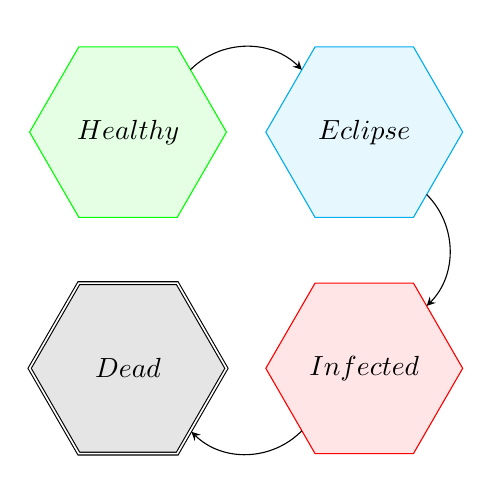
\begin{tikzpicture}[
        Healthy/.style={regular polygon,regular polygon sides=6, draw, minimum size=2.5cm, inner sep=0pt, outer sep=0pt, draw=AGreen, fill=AGreen!10},
        Eclipse/.style={regular polygon,regular polygon sides=6, draw, minimum size=2.5cm, inner sep=0pt, outer sep=0pt, draw=cyan, fill=cyan!10},
        Infected/.style={regular polygon,regular polygon sides=6, draw, minimum size=2.5cm, inner sep=0pt, outer sep=0pt, draw=red, fill=red!10},
        Dead/.style={regular polygon,regular polygon sides=6, draw, minimum size=2.5cm, inner sep=0pt, outer sep=0pt, draw=black, fill=black!10}]

        \node[Healthy] (H) {$Healthy$};
        \onslide<4->{\node[Eclipse, right of=H] (E) {$Eclipse$};}
        \onslide<5->{\node[Infected, below of=E] (I) {$Infected$};}
        \onslide<6->{\node[Dead, accepting, below of=H] (D) {$Dead$};}
            
        \onslide<4->{\draw   (H) edge[bend left=45] node [above] {} (E);}
        \onslide<5->{\draw   (E) edge[bend left=45] node [right] {} (I);}
        \onslide<6->{\draw   (I) edge[bend left=45] node [below] {} (D);}

%        \draw   (H) edge[bend left=45] node [above] {Infection event} (E);
%        \draw   (E) edge[bend left=45] node [right] {UT $>$ HT + ET} (I);
%        \draw   (I) edge[bend left=45] node [below] {UT $>$ HT + ET + IT} (D);

%        \draw   (H) edge[bend right=45] node [below left] {} (E);
%        \draw   (E) edge[bend right=45] node [below left] {$\tau_E$} (I);
%        \draw   (I) edge[bend right=45] node [below left] {$\tau_I$} (D);
    \end{tikzpicture}}
    \end{center}}}}
\column{0.5\textwidth}
    \onslide<8->{%
    \fbox{\parbox{\textwidth}{%
    \vspace{2.5em}
    \begin{center}
    Minimize the SSR
    $$\mathrm{SSR} = \sum_{i=1}^{n} (y_i - \hat y_i)^{2}$$
    \end{center}
    \vspace{2.5em}}}}
\end{columns}}
\end{center}
\end{frame}

%-----------------------------------------------------------------------------------
\section{Results}

\begin{frame}{Full Dish}
\begin{center}
\resizebox{1.0\linewidth}{!}{%
\begin{columns}[T]
\column{0.5\textwidth}
    \begin{center}
    Cells
    \end{center}
\column{0.5\textwidth}
    \begin{center}
    Virus
    \end{center}
\end{columns}}

\resizebox{1.0\linewidth}{!}{%
\begin{columns}[T]
\column{0.50\textwidth}
    \begin{center}
%    \only<2->{\resizebox{1.0\textwidth}{!}{\animategraphics[autoplay]{20}{Full-Dish-CellPhotos/cell}{0}{140}}}
    \only<1>{\resizebox{1.0\linewidth}{!}{\includegraphics{Full-Dish-CellPhotos/cell0.png}}}
    \end{center}

\column{0.50\textwidth}
    \begin{center}
%    \only<2->{\resizebox{1.0\textwidth}{!}{\animategraphics[autoplay]{20}{Full-Dish-VirusPhotos/virus}{0}{140}}}
    \only<1>{\resizebox{1.0\linewidth}{!}{\includegraphics{Full-Dish-VirusPhotos/virus0.png}}}
    \end{center}    

\end{columns}}
\end{center}
\end{frame}

\begin{frame}{Single Plaque}
\begin{center}
\resizebox{1.0\linewidth}{!}{%
\begin{columns}[T]
\column{0.5\textwidth}
    \begin{center}
    Cells
    \end{center}
\column{0.5\textwidth}
    \begin{center}
    Virus
    \end{center}
\end{columns}}

\resizebox{1.0\linewidth}{!}{%
\begin{columns}[T]
\column{0.50\textwidth}
    \begin{center}
%    \only<2->{\resizebox{1.0\textwidth}{!}{\animategraphics[autoplay]{20}{Zoomed-In-CellPhotos/cell}{0}{90}}}
    \only<1>{\resizebox{1.0\linewidth}{!}{\includegraphics{Zoomed-In-CellPhotos/cell0.png}}}
    \end{center}

\column{0.50\textwidth}
    \begin{center}
%    \only<2->{\resizebox{1.0\textwidth}{!}{\animategraphics[autoplay]{20}{Zoomed-In-VirusPhotos/virus}{0}{90}}}
    \only<1>{\resizebox{1.0\linewidth}{!}{\includegraphics{Zoomed-In-VirusPhotos/virus0.png}}}
    \end{center}    

\end{columns}}
\end{center}
\end{frame}

\begin{frame}{Experiment vs Simulation}
\begin{center}
\resizebox{1.0\linewidth}{!}{%
\begin{columns}[T]
\column{0.5\textwidth}
    \begin{center}
    Experiment
    \end{center}
\column{0.5\textwidth}
    \begin{center}
    Simulation
    \end{center}
\end{columns}}

\resizebox{1.0\linewidth}{!}{%
\begin{columns}[T]
\column{0.50\textwidth}
    \begin{center}
    \onslide<2->{\resizebox{1.0\linewidth}{!}{\includegraphics{plaques}}}
    \end{center}

\column{0.50\textwidth}
    \begin{center}
    \onslide<3->{\resizebox{1.0\linewidth}{!}{\includegraphics{Full-Dish-CellPhotos/cell55.png}}}
    \end{center}    
\end{columns}}
\end{center}
\end{frame}

\begin{frame}{Speed Up}
    \begin{center}
    \only<1->{\resizebox{0.7\linewidth}{!}{\includegraphics{loglogspeed}}}
    \end{center}  
\end{frame}

\begin{frame}{Data Fitting}
    \begin{center}
    \only<1->{\resizebox{0.7\linewidth}{!}{\includegraphics{DataFit}}}
    \end{center}  
\end{frame}

\begin{frame}{Data Fitting Parameters}
\begin{center}
\resizebox{1.0\linewidth}{!}{%
\begin{tabular}{llc}
\hline
Parameter & Meaning & Value \\
\hline
$\beta$ & Infection rate & 53.64 $/\mathrm{h}$ \\
$p$ & Viral production rate & 3005.05 $/\mathrm{h}$ \\
$c$ & Viral clearance rate & 0.25 $/\mathrm{h}$ \\
$D$ & Diffusion coefficient & 2.16$\times 10^{-8}$ $\mathrm{m}^2/\mathrm{h}$ (fixed) \\
$\tau_E$ & Mean eclipse duration & 15.87 $\mathrm{h}$ \\
$\eta_E$ & Eclipse shape parameter & 30 (fixed) \\
$\tau_I$ & Mean infectious lifespan & 26.19 $\mathrm{h}$ \\
$\eta_I$ & Infectious shape parameter & 100 (fixed) \\
\end{tabular}}
\end{center}  
\end{frame}

%-----------------------------------------------------------------------------------
\miniframesoff
\section{}

\begin{frame}{Acknowlegdements}

    \begin{itemize}
        \item<2-> Dr. Hana M. Dobrovolny
        \item<2-> Dr. Gilberto Gonzalez-Parra
    \end{itemize}

\end{frame}

\begin{frame}{}

\begin{center}
\Huge Thank You
\end{center}

\end{frame}


\miniframesoff
\section{}

%Extra
\begin{frame}{}
    %Blank
\end{frame}

\begin{frame}{Diffusion limit}
    $$\Delta t \le \frac{1}{2}\frac{(\Delta x)^2}{D}$$
    $$\Delta t \le 0.05787 h$$
\end{frame}

\begin{frame}{Clusters/Servers vs GPUs}
    AWS - 70 TFLOPS
\end{frame}

\begin{frame}[fragile]{More specific example of Using the GPUs}
\vspace{0.5em}
\resizebox{1.0\linewidth}{!}{%
\begin{columns}[c]
\column{0.5\textwidth}
    \begin{center}
        \texttt{CPU}
    \end{center}
\column{0.5\textwidth}
    \begin{center}
        \texttt{GPU}
    \end{center}
\end{columns}}
\vspace{-3em}

\begin{columns}[T]
\column{0.5\textwidth}
    \begin{center}
    \begin{lstlisting}[style=CStyle]
    array = (float**) calloc(1792,sizeof(float*));
    for(int i=0; i<sizeof(array)/sizeof(array[0]); i++){
        array[i] = array[i] + 1;
    }
    \end{lstlisting}
    \end{center}
\column{0.5\textwidth}
    \begin{center}
    \begin{lstlisting}[style=CStyle]
    array = (float**) calloc(1792,sizeof(float*));
    cudaMalloc((void**)&array_GPU, 1792*sizeof(float));
    
    cudaMemcpy( array_GPU, array, 1792*sizeof(float), cudaMemcpyHostToDevice);
    array_GPU[id] = array_GPU[id] + 1;
    cudaMemcpy( array, array_GPU, 1792*sizeof(float), cudaMemcpyDeviceToHost);
    \end{lstlisting}
    \end{center}
\end{columns}
\end{frame}

\end{document}
